\documentclass[11pt]{article}
\usepackage{fullpage}
\usepackage{graphicx}
\usepackage[section]{placeins}
\usepackage{indentfirst}
\usepackage{enumitem}
\usepackage{listings}

\title{Beating Chessmasters with a Computer}

\author{
Bart Kerfeld\\kerfe010@umn.edu
}
\date{\today}



\begin{document}
\lstset{xleftmargin=\parindent}
\maketitle

\begin{abstract}
Computer chess has, for the last century, been a passion of many people interested in the field of artificial intelligence. During that time, those people have developed and iterated upon several different approaches. Recently, the best of these approaches combined with the advancements in computer processing power has allowed chess programs to become better than the best human players. This paper attempts to explain the way that these programs work starting at a high level and working down to the implementation details (focusing mostly on the strongest known approaches). From there, I showcase my own relatively simple engine, BKChess, which utilizes many the discussed approaches and put it through some tests to measure its strength. 
\end{abstract}

\vspace{1cm}

\begin{center}
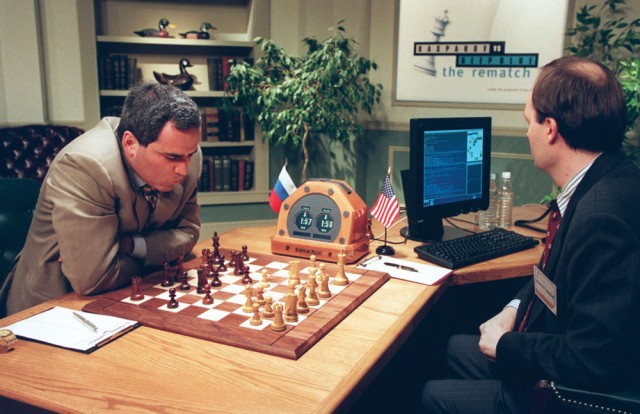
\includegraphics[scale=0.55]{kasparov-vs-ibm-deep-blue-640x414.jpg}
\linebreak
Grandmaster Garry Kasparov facing IBM's Deep Blue\cite{anthony_2014}.
\end{center}

\clearpage

\section{Introduction}
The game of chess is a popular board game that has been around for over a thousand years. It is played with two players on an eight by eight checkered game-board. Both players begin with sixteen total pieces consisting of six different types: eight pawns, two rooks, two knights, two bishops, one queen and one king. Each of these piece types can be moved in its own unique way. The players alternate turns moving one piece at a time with the goal of trying to capture his or her opponent's king and win the game. In order to be played well, the game requires the players to think several moves ahead by visualize several move variations. 

Designing a computer program to play chess has been thought about by mathematicians and computer scientists for well over a century. It is a difficult problem because the number of unique states is too large to deterministically solve it. Instead, the program needs to combine elements of artificial intelligence, including heuristic-based search, with efficient data structures to find good moves in a reasonable amount of time.

\section{A High Level Look}
Before diving into the details of the methods used to make strong engines, I think it is necessary to first understand, at a high level, the fundamentals needed to make one function. To construct a program capable of playing reasonable chess, the following four things are needed:

\begin{itemize}[noitemsep]
  \item Board Structure
  \item Move Generator
  \item Move Searcher
  \item Position Evaluator
\end{itemize}

The \textbf{Board Structure} is the foundation that on which the engine stands. It holds information about the location of the pieces, the castle permissions for each side, the number of times a position has occurred, the number of moves since the last piece capture or pawn move, and the current side to move \cite{bovskovic2005representation, shannon1950xxii}. Sitting on top of this structure is the \textbf{Move Generator}. This component uses the information from the board structure to generate all legal moves for the current side to play. With the capability to generate all legal moves from any position, the \textbf{Move Searcher} explores different variations trying to find the one with the greatest winning chances. Because there are too many variations to exhaustively search, a \textbf{Position Evaluator} is needed to act as a heuristic to guide the search. This component looks only at the information from the current position and assigns a numeric value corresponding to how favorable the position is. With this, the Move Searcher can avoid searching to the roots of the game tree and also, if done cleverly, can avoid searching many move variations altogether (more on that later). Using these four components in an efficient manner, a computer program can be written to play reasonable chess. Now that that the basics have been presented, we can move on to the more interesting details in the following sections.

\section{Board Representation}
The location of the pieces on the board at any given state is undeniably important. In order for any sort of evaluation or search to take place, the location of the pieces must be constantly checked and updated. Because it is necessary to evaluate and search through millions of positions to ensure the computer can make good moves, it is critical that the structure used is fast and reliable. 

Over the years, many different methods have been tested. The earliest and most natural of these is to use a two-dimensional eight by eight array to store a value at each index representing the piece on the board. While this method is easy to understand and implement, it is relatively slow since it requires lots of looping and memory accesses\cite{bovskovic2005representation}. A better representation is to use a set of 64-bit integers called bitboards. With this representation, each bit in the bitboard corresponds to a square on the 64-square chessboard. Using just 12 bitboards (six for each piece, each with two possible colors), the position of all pieces can be encoded \cite{segundo2006efficient}. Not only is the amount of space needed small for this representation, but it also allows for very quick evaluation functions. Consider, for example, that you wish to check if there are any white pawns on the seventh rank. To do this with the bitboard model, one simply must logically AND the white pawn bitboard with a precomputed bitboard containing 1 bits in all rank seven locations and 0 bits elsewhere. If the result is nonzero, then there is a pawn on the seventh rank, and if it is zero there is not. In contrast, the same check using the eight by eight array model would involve having to loop through all squares on rank seven and check if any are set to the value of a white pawn. This would involve eight equality checks and seven increments to the array index. Although this example is contrived, it still makes clear the advantages bitboards provide especially when trying to compute information about multiple pieces or squares. Not surprisingly, the current top-ranked chess engine in the world, Stockfish, uses the bitboard model to represent its pieces.

\section{Search} %\cite{schaeffer1989history} 
The basic and most widely used search mechanism used in chess programs is iterative deepening alpha-beta search\cite{reinefeld1983improvement}. This is standard alpha-beta with cutoffs except that rather than go to leaf nodes of the game tree, it stops at a certain depth and uses the evaluation function to measure the strength of the node.  Often, this is implemented in the framework of NegaMax so a single function can be used (rather than both an alphaBetaMax and alphaBetaMin for white and black respectively)\cite{boule2002fpga}. The code for this might look as follows (c-like pseudocode):

\begin{lstlisting}
int alphaBeta(int alpha, int beta, int depthleft) {
  if (depthleft == 0) {
    return EvalPos();
  }
  for ( all legal moves ) {
    score = -alphaBeta(-beta, -alpha, depthleft - 1);
    if (score >= beta) {
      return beta;
    }
    if (score >= alpha) {
      alpha = score;
    }
  }
  return alpha;
}
\end{lstlisting}

Using an iterative deepening version of this has a couple of advantages. The first is that the engine will always to have a move to play even if it is interrupted. This is because the best move will be updated at each iteration. For example, if the engine was interrupted while trying to perform alpha-beta to depth 5, it still has its known result from alpha-beta depth 4 to return. The second is that it allows the searches at higher depths to prune more nodes by first searching the best move from the previous depth. This is because the best move from the previous depth is likely still a good move at the current one, and better moves prune more nodes. Due to the significance of both of these things, nearly all chess engines search using the iterative deepening approach.

This method alone, however has a few issues which leave room for improvement. First, it does not account for the case where one move after the end of the search the opponent can make a winning move such as taking a piece. Consider an example where at the end of the search tree, the "best move" computed is to take the opponent knight with a queen. A simple evaluation would think this looks good since a piece was captured at no cost, however, the search fails to consider that the opponent may be able to capture our queen immediately on the next move. This problem is known as the horizon effect \cite{tabibi2002verified}. To counteract this, we perform a quiescence search at all leaves of the alpha-beta search. The quiescence search performs a  limited version of alpha-beta but rather than search all moves to a certain depth, it searches only capture moves until the position it reaches is stable. The second issue with the alpha-beta search is that it re-searches the same position multiple times. For example, say the moves of one branch of the tree are pawn e4, pawn e5, knight f3 and the second branch are knight f3, pawn e5, pawn e4. The resulting position of both branches is the same, yet alpha-beta as written will spend time searching through both branches. The remedy for this issue is a transposition table, which is simply a hash table indexed using a position dependent hash function. Every time a position is searched, an entry is added to the table containing the result of the search, the move that led to that value (aka the best move) and the depth to which the tree was searched \cite{schaeffer1989history}. With this information, some re-searching can be avoided causing an overall speed up in search. Using these two extensions to alpha-beta, the engine is capable of searching to a reasonable depth and avoid horizon effects.

\section{Evaluation} 
Ultimately the strength of a chess program comes down to its ability to evaluate a position. "While search techniques are pretty much universal and move generation can be deducted from the game's rules and no more, evaluation requires a deep and thorough analysis of strategy\cite{laramee2000chess}." The final section discusses some things to consider when writing evaluation functions.

Obviously, one of the most promising indicators of a good position is the amount of pieces you have compared to the number of pieces your opponent has. This is referred to as the material score. Each piece is assigned a value. If the sum over all pieces multiplied by their respective value is greater for one player than the other, than that player is said to have a material advantage. This seems like such a simple measure, but its importance is undeniable. Creators of the powerful Chess 4.5 program estimate that an enormous advantage in other aspects of the game such is position, mobility , and safety is worth no more than one and a half pawns (the piece worth the least material)\cite{laramee2000chess}. That said, these other aspects are what separate the good programs from the great. The best engines consider things like pawn formations, king safety, and development. The tricky thing about evaluation is it is impossible to know whether or not you have a good one without testing, it is trial and error. Generally speaking though, it is best to keep your evaluation simple to allow deeper searching. "It is very difficult to refine an evaluation function enough to gain as much performance as an extra ply (half-move) of search\cite{laramee2000chess}."

\section{BKChess}
Now that some of the methods for developing chess engines have been discussed, it is time to move on to my own approach, specifically the engine I created called BKChess. The engine is written entirely in C++, and it utilizes many of the ideas mentioned earlier. The primary focus when developing BKChess was on fast move generation and pruning the search tree as much as possible, since the search tree is the primary artificial intelligence element. I wanted to do all this while keeping the program fairly simple and easy to read. In this section, I will discus how the four components designed to achieve these ends.

Beginning with the board representation and move generator, I decided to start by using the bitboard model discussed earlier to represent all the pieces. The bitboards are stored in an array inside a Board class which also contains information about the side to play, the fifty move rule, the three-move repetition rule, the castle permissions and the enPassant square (if any). With the help of some existing code\cite{bitboards}, I was able to create lookup tables on initialization which the engine was then able to use to quickly compute all of the legal moves for any given piece on any given square. This combined with a couple brute-force checks for the legality of special moves such as enPassant and castle allow for a reasonably quick move generator (approximately one million moves per second on my laptop). 

Moving on the searcher, I used the gold standard iterative deepening alpha-beta with quiescence search discussed earlier. The interesting part is the order it searches the moves. The first move searched is always the principle variation, the best move from the search at the previously level in the iterative deepening as this is most often the best move. Next, it looks at all capture moves in the order of most value victim, least valuable attacker (i.e. pawn takes queen is searched before queen takes pawn as it is generally a better move). After the principle move and all capture moves have been searched, the next moves looked at are those which caused a beta cutoff in the previous search. These moves are called killer moves. These moves are good moves, by definition, since they caused the search to avoid a branch. The next tier of moves searched are those which cause alpha-cutoffs for much the same reasoning as the killer moves. Finally, the remaining moves are searched. Using these orderings, the number of nodes needed to be searched was dropped dramatically. 

Finally, the last component of the engine is the evaluation function. As it was not the primary focus of my engine, I kept it strikingly simple using a simple function I found online\cite{BluefeverSoftware}. First the material score is calculated by taking the number of pieces of each type each player has an multiplying them by the following constants: 100 for pawn, 325 for knight, 325 for bishop, 550 for rook, 1000 for queen and 50000 for king. Then a sum was computed for the white and black players and the difference is the score. This alone, resulted in the engine playing very passively so it also factors in the location of the pieces to reward development. This is simply a bonus for having different pieces located on different squares. The bonus amount comes from tables which look like the following: (I have shown the tables for white, the black is just a mirror)

\begin{center}
\begin{tabular}{c c c c c c c c c}
\textbf{8} & 0  & 0  & 0  & 0  & 0  & 0  & 0  & 0  \\
\textbf{7} & 20 & 20 & 20 & 30 & 30 & 20 & 20 & 20 \\
\textbf{6} & 10 & 10 & 10 & 20 & 20 & 10 & 10 & 10 \\
\textbf{5} & 5  & 5  & 5  & 10 & 10 & 5  & 5  & 5  \\
\textbf{4} & 0  & 0  & 10 & 20 & 20 & 10 & 0  & 0  \\
\textbf{3} & 5  & 0  & 0  & 5  & 5  & 0  & 0  & 5  \\
\textbf{2} & 10 & 10 & 0  &-10 &-10 & 0  & 10 & 10 \\
\textbf{1} & 0  & 0  & 0  & 0  & 0  & 0  & 0  & 0  \\
  & \textbf{A}  & \textbf{B}  & \textbf{C}  & \textbf{D}  & \textbf{E}  & \textbf{F}  & \textbf{G}  & \textbf{H}
\end{tabular} \\
Pawn Table
\end{center} 

\begin{center}
\begin{tabular}{c c c c c c c c c}
\textbf{8} & 0  & 0  & 0  & 0  & 0  & 0  & 0  & 0  \\
\textbf{7} & 0  & 0  & 0  & 10 & 10 & 0  & 0  & 0 \\
\textbf{6} & 5  & 10 & 10 & 20 & 20 & 10 & 10 & 5 \\
\textbf{5} & 5  & 10 & 15 & 20 & 20 & 15 & 10 & 5  \\
\textbf{4} & 0  & 0  & 10 & 20 & 20 & 10 & 0  & 0  \\
\textbf{3} & 0  & 0  & 10 & 10 & 10 & 10 & 0  & 0  \\
\textbf{2} & 0  & 0  & 0  & 5  & 5  & 0  & 0  & 0 \\
\textbf{1} & 0  &-10 & 0  & 0  & 0  & 0  &-10 & 0  \\
  & \textbf{A}  & \textbf{B}  & \textbf{C}  & \textbf{D}  & \textbf{E}  & \textbf{F}  & \textbf{G}  & \textbf{H}
\end{tabular} \\
Knight Table
\end{center} 

\begin{center}
\begin{tabular}{c c c c c c c c c}
\textbf{8} & 0  & 0  & 0  & 0  & 0  & 0  & 0  & 0  \\
\textbf{7} & 0  & 0  & 0  & 10 & 10 & 0  & 0  & 0 \\
\textbf{6} & 0  & 0  & 10 & 15 & 15 & 10 & 0  & 0 \\
\textbf{5} & 0  & 10 & 15 & 20 & 20 & 15 & 10 & 0  \\
\textbf{4} & 0  & 10 & 15 & 20 & 20 & 15 & 10 & 0  \\
\textbf{3} & 5  & 0  & 10 & 15 & 15 & 10 & 0  & 5  \\
\textbf{2} & 0  & 0  & 0  & 10 & 10 & 0  & 0  & 0 \\
\textbf{1} & 0  & 0  &-10 & 0  & 0  &-10 & 0  & 0  \\
  & \textbf{A}  & \textbf{B}  & \textbf{C}  & \textbf{D}  & \textbf{E}  & \textbf{F}  & \textbf{G}  & \textbf{H}
\end{tabular} \\
Bishop Table
\end{center}

\begin{center}
\begin{tabular}{c c c c c c c c c}
\textbf{8} & 0  & 0  & 5  & 10 & 10 & 5  & 0  & 0  \\
\textbf{7} & 25 & 25 & 25 & 25 & 25 & 25 & 25 & 25 \\
\textbf{6} & 10 & 10 & 10 & 20 & 20 & 10 & 10 & 10 \\
\textbf{5} & 0  & 0  & 5  & 10 & 10 & 5  & 0  & 0  \\
\textbf{4} & 0  & 0  & 5  & 10 & 10 & 5  & 0  & 0  \\
\textbf{3} & 0  & 0  & 5  & 10 & 10 & 5  & 0  & 0  \\
\textbf{2} & 0  & 0  & 5  & 10 & 10 & 5  & 0  & 0  \\
\textbf{1} & 0  & 0  & 5  & 10 & 10 & 5  & 0  & 0  \\
  & \textbf{A}  & \textbf{B}  & \textbf{C}  & \textbf{D}  & \textbf{E}  & \textbf{F}  & \textbf{G}  & \textbf{H}
\end{tabular} \\
Rook Table
\end{center} 

With these tables added to the evaluation function, the engine is rewarded by developing its pieces to good squares. Notice, however, that the weights are all less than the material. For this reason, the engine will never elect to give up material in exchange for getting a piece on a good square. This is not always a best idea, but more often than not it is. Because this engine is intentionally simple, I decided it would be sufficient for my goals.

\section{Testing its Strength}
Having spent the time to build the engine, I naturally wanted to get an idea of how strong it was. So I installed the chess GUI Areana 3.5.1 using wine on Ubuntu as well as three other engines which I predicted would have similar strength. From there, I set up a tournament where BKChess played each of these engines as well as myself ten games each (a total of 40 games). Each player had a total of five minutes to play and received a one second increment every time a move was played. The results of this series are shown in the figure below:

\begin{center}
\begin{tabular}{c c c c c}
\textbf{Opponent} & \textbf{Opponent Rating} & \textbf{Wins} & \textbf{Losses} & \textbf{Draws} \\
Me         & 1111 & 6 & 2 & 2 \\
SUPRA 12.0 & 1201 & 6 & 4 & 0 \\
Nero61     & 1428 & 5 & 3 & 2 \\
SEE069     & 1702 & 1 & 8 & 1
\end{tabular}
\end{center}

My rating is based on 915 blitz games played on Chess.com against other human players and the engine rankings are based on an excess of 2000 games against different engines\cite{computerchess}.

%Bkchess - Bart(me)			: 7.0/10 6-2-2 (1111=101=1)
%Bkchess - Nero_61          : 6.5/10 5-3-2 (10=0=11110)
%Bkchess - SEE069           : 1.5/10 1-8-1 (00100000=0)
%Bkchess - SUPRA 12.0 32bit : 5.0/10 5-5-0 (1010101010)

As can be seen BKChess competes fairly well at this level. Using the FIDE initial ratings calculator, BKChess has an estimated rating of 1406 which is superior to that of an average chess player. It, however, comes no where close to master level (2200), grandmaster level (2500) or top engine level (3200). In the following section, I will discus a few of the improvements that could be made in the future to improve the performance so that it could compete at these higher levels.

\section{Improving the Engine}
The most glaringly obvious thing that would benefit the engine is a better evaluation function. There are several heuristics in chess which can be computed quickly such as pawn structure and king safety that the engine does not consider at all. This would be the quickest and easiest modification that would dramatically improve the engine. The next thing I would do is incorporate a transposition table to avoid having to re-search the same position from multiple position. This would likely increase the depth of the search by one or two levels significantly improving the performance of the engine. Finally, I would incorporate an opening book by storing the best known openings to help achieve good positions. If I decide to continue working on the engine these are the first three things I would implement. With them, I do not think the engine would lose against any of the opponents showcased in the previous section. 

\section{Conclusion}
At a high level, a chess engine seems like a fairly simple program. It simply stores the information of the game, generates and searches through the legal moves and evaluates the best course of action to take. Having looked closer at the details by implementing my own engine, I think it is safe to say this is not the case. There are several edge cases to consider, many positions to search and many different evaluation strategies and heuristics to implement. On top of this, it is difficult to get quick feedback on the performance of the engine as is must play several games with reasonable time control before any reasonable conclusions can be reached. This dramatically impacts the speed at which the engine can be iterated. Despite these difficulties, thanks to the help of many smart people, computers have been taught to play chess at an incredibly high level. So high, that computers are now in fact the best known chess players in the universe!

\vspace{\fill}

\bibliographystyle{abbrv}
\bibliography{./bkchess.bib}

\end{document}


